% !TEX root = ../../main.tex

\chapter{Random Rate Networks and SCS Chaos}
\label{ch:random-rate-networks-scs-chaos}

\section*{What This Chapter Adds}

The previous chapters built up the pieces of clustered spiking networks: single
neurons, filtered spike trains, population rates, balanced excitation and
inhibition, and clustered attractors. We now temporarily simplify the
microscopic picture. Instead of tracking every spike time, we study recurrent
rate equations whose variables are continuous population activities. This is not
a claim that spikes are irrelevant. It is a controlled change of language: rate
models isolate the deterministic feedback mechanisms that can create
macroscopic chaos, while the spiking model later tells us how those effective
variables, noise levels, and time constants arise.

The central example is the Sompolinsky--Crisanti--Sommers (SCS) random rate
network. It shows that a high-dimensional recurrent system can pass from a
stable fixed point to irregular deterministic activity when the recurrent gain
crosses a critical value. That transition is the conceptual template for the
course's later question of whether paired excitatory/inhibitory clusters can
behave like effective rate units whose quenched inter-cluster variability
produces mesoscopic chaos.

\section{From Spikes to Effective Rate Variables}
\label{sec:ch06-rate-variables}

Let \(x_i(t)\) denote the input, membrane-potential-like drive, or activation
variable of an effective unit \(i\). Its firing rate is modeled as
\[
        r_i(t) = \phi(x_i(t)),
\]
where \(\phi\) is a static transfer function. The function \(\phi\) summarizes
the input-output curve of a neuron, population, or cluster: large input gives a
larger output rate, while saturation and refractoriness keep the rate finite.
In a recurrent rate network the activity obeys
\[
        \tau_r \frac{d x_i}{dt}
        =
        -x_i(t) + \sum_{j=1}^{N} J_{ij}\,\phi(x_j(t)) + I_i .
        \label{eq:ch06-basic-rate-network}
\]
Here \(N\) is the number of effective units, \(\tau_r\) is the relaxation time of
the rate variable, \(J_{ij}\) is the coupling from unit \(j\) to unit \(i\), and
\(I_i\) is a constant external drive. The term \(-x_i\) says that input decays
without recurrent support. The sum says that the present state of the network
is fed back through the nonlinearity \(\phi\).

Equation~\eqref{eq:ch06-basic-rate-network} is the rate analogue of filtered
spiking input. In the spiking model, spike trains \(s_i(t)\) are convolved with
a synaptic kernel. In the rate model, \(\phi(x_j(t))\) is already the smoothed
output of the effective unit. This is why rate equations are natural for cluster
activities \(r_\alpha(t)\): a cluster rate is a filtered, averaged object, not a
single spike train.

\section{Random Recurrent Coupling}
\label{sec:ch06-random-coupling}

The SCS model chooses the recurrent couplings to be random with zero mean,
\[
        J_{ij} = \frac{g}{\sqrt{N}}\,\chi_{ij},
        \label{eq:ch06-scs-couplings}
\]
where the random variables \(\chi_{ij}\) are independent with mean \(0\) and
variance \(1\). The parameter \(g\) is the coupling strength. The factor
\(1/\sqrt{N}\) is essential: each unit receives \(N\) inputs, and this scaling
keeps the net random input of order one as \(N\) grows.

The simplest deterministic state is a homogeneous fixed point. With \(I_i=0\)
and an odd transfer function such as \(\phi(x)=\tanh(x)\), \(x_i=0\) for all
\(i\) is a fixed point. To test its stability, perturb it by a small vector
\(\delta x\). Since \(\phi(x)\approx \phi'(0)x\) near zero,
\[
        \tau_r \frac{d\,\delta x}{dt}
        =
        \left[-I_N + \phi'(0)J\right]\delta x .
        \label{eq:ch06-linearized-rate}
\]
The identity matrix \(I_N\) contributes decay. The matrix \(J\) contributes
recurrent amplification. For a large random matrix of the
form~\eqref{eq:ch06-scs-couplings}, its eigenvalues fill a disk whose radius is
approximately \(g\). Thus the fixed point is linearly stable when
\[
        g\,\phi'(0) < 1
\]
and loses stability when the random recurrent amplification overcomes leak.
For the standard normalization \(\phi'(0)=1\), the critical value is
\[
        g_c = 1 .
        \label{eq:ch06-scs-critical-g}
\]

This is the first diagnostic of the SCS transition: below \(g_c\), small
perturbations contract; above \(g_c\), at least some perturbation directions
expand. The nonlinear transfer function prevents indefinite growth, so the
post-transition state is not simply divergent. It becomes irregular, bounded,
high-dimensional motion.

The same calculation should be reused whenever a cluster-level model is
proposed. Linearize the deterministic mesoscopic equations, isolate the random
inter-cluster block, and compare its effective spectral radius with leak and
local damping. For a scalar cluster reduction
\[
        \tau_c \dot u_a
        =
        -u_a+\sum_b W_{ab}\Phi(u_b)+I_a,
\]
the tangent dynamics around a state \(u(t)\) contains
\[
        \tau_c \dot{\delta u}_a
        =
        -\delta u_a+
        \sum_b W_{ab}\Phi'(u_b(t))\delta u_b .
        \label{eq:ch06-local-gain-cluster}
\]
If the off-diagonal block has row variance \(\sigma_W^2/Q\), the instantaneous
random gain is estimated by
\[
        \rho_{\mathrm{eff}}(t)
        \approx
        \sigma_W
        \sqrt{\left\langle q_b^2(t)\right\rangle_b},
        \qquad
        q_b(t)=\Phi^{\prime}(u_b(t)).
        \label{eq:ch06-effective-spectral-radius}
\]
This is not a proof of chaos in the spiking network. It is a diagnostic target:
if \(\rho_{\mathrm{eff}}\) is far below one, SCS-like rate chaos is unlikely; if
it is near or above one, autocorrelation and Lyapunov tests become the right
next measurements.

\begin{figure}[htbp]
    \centering
    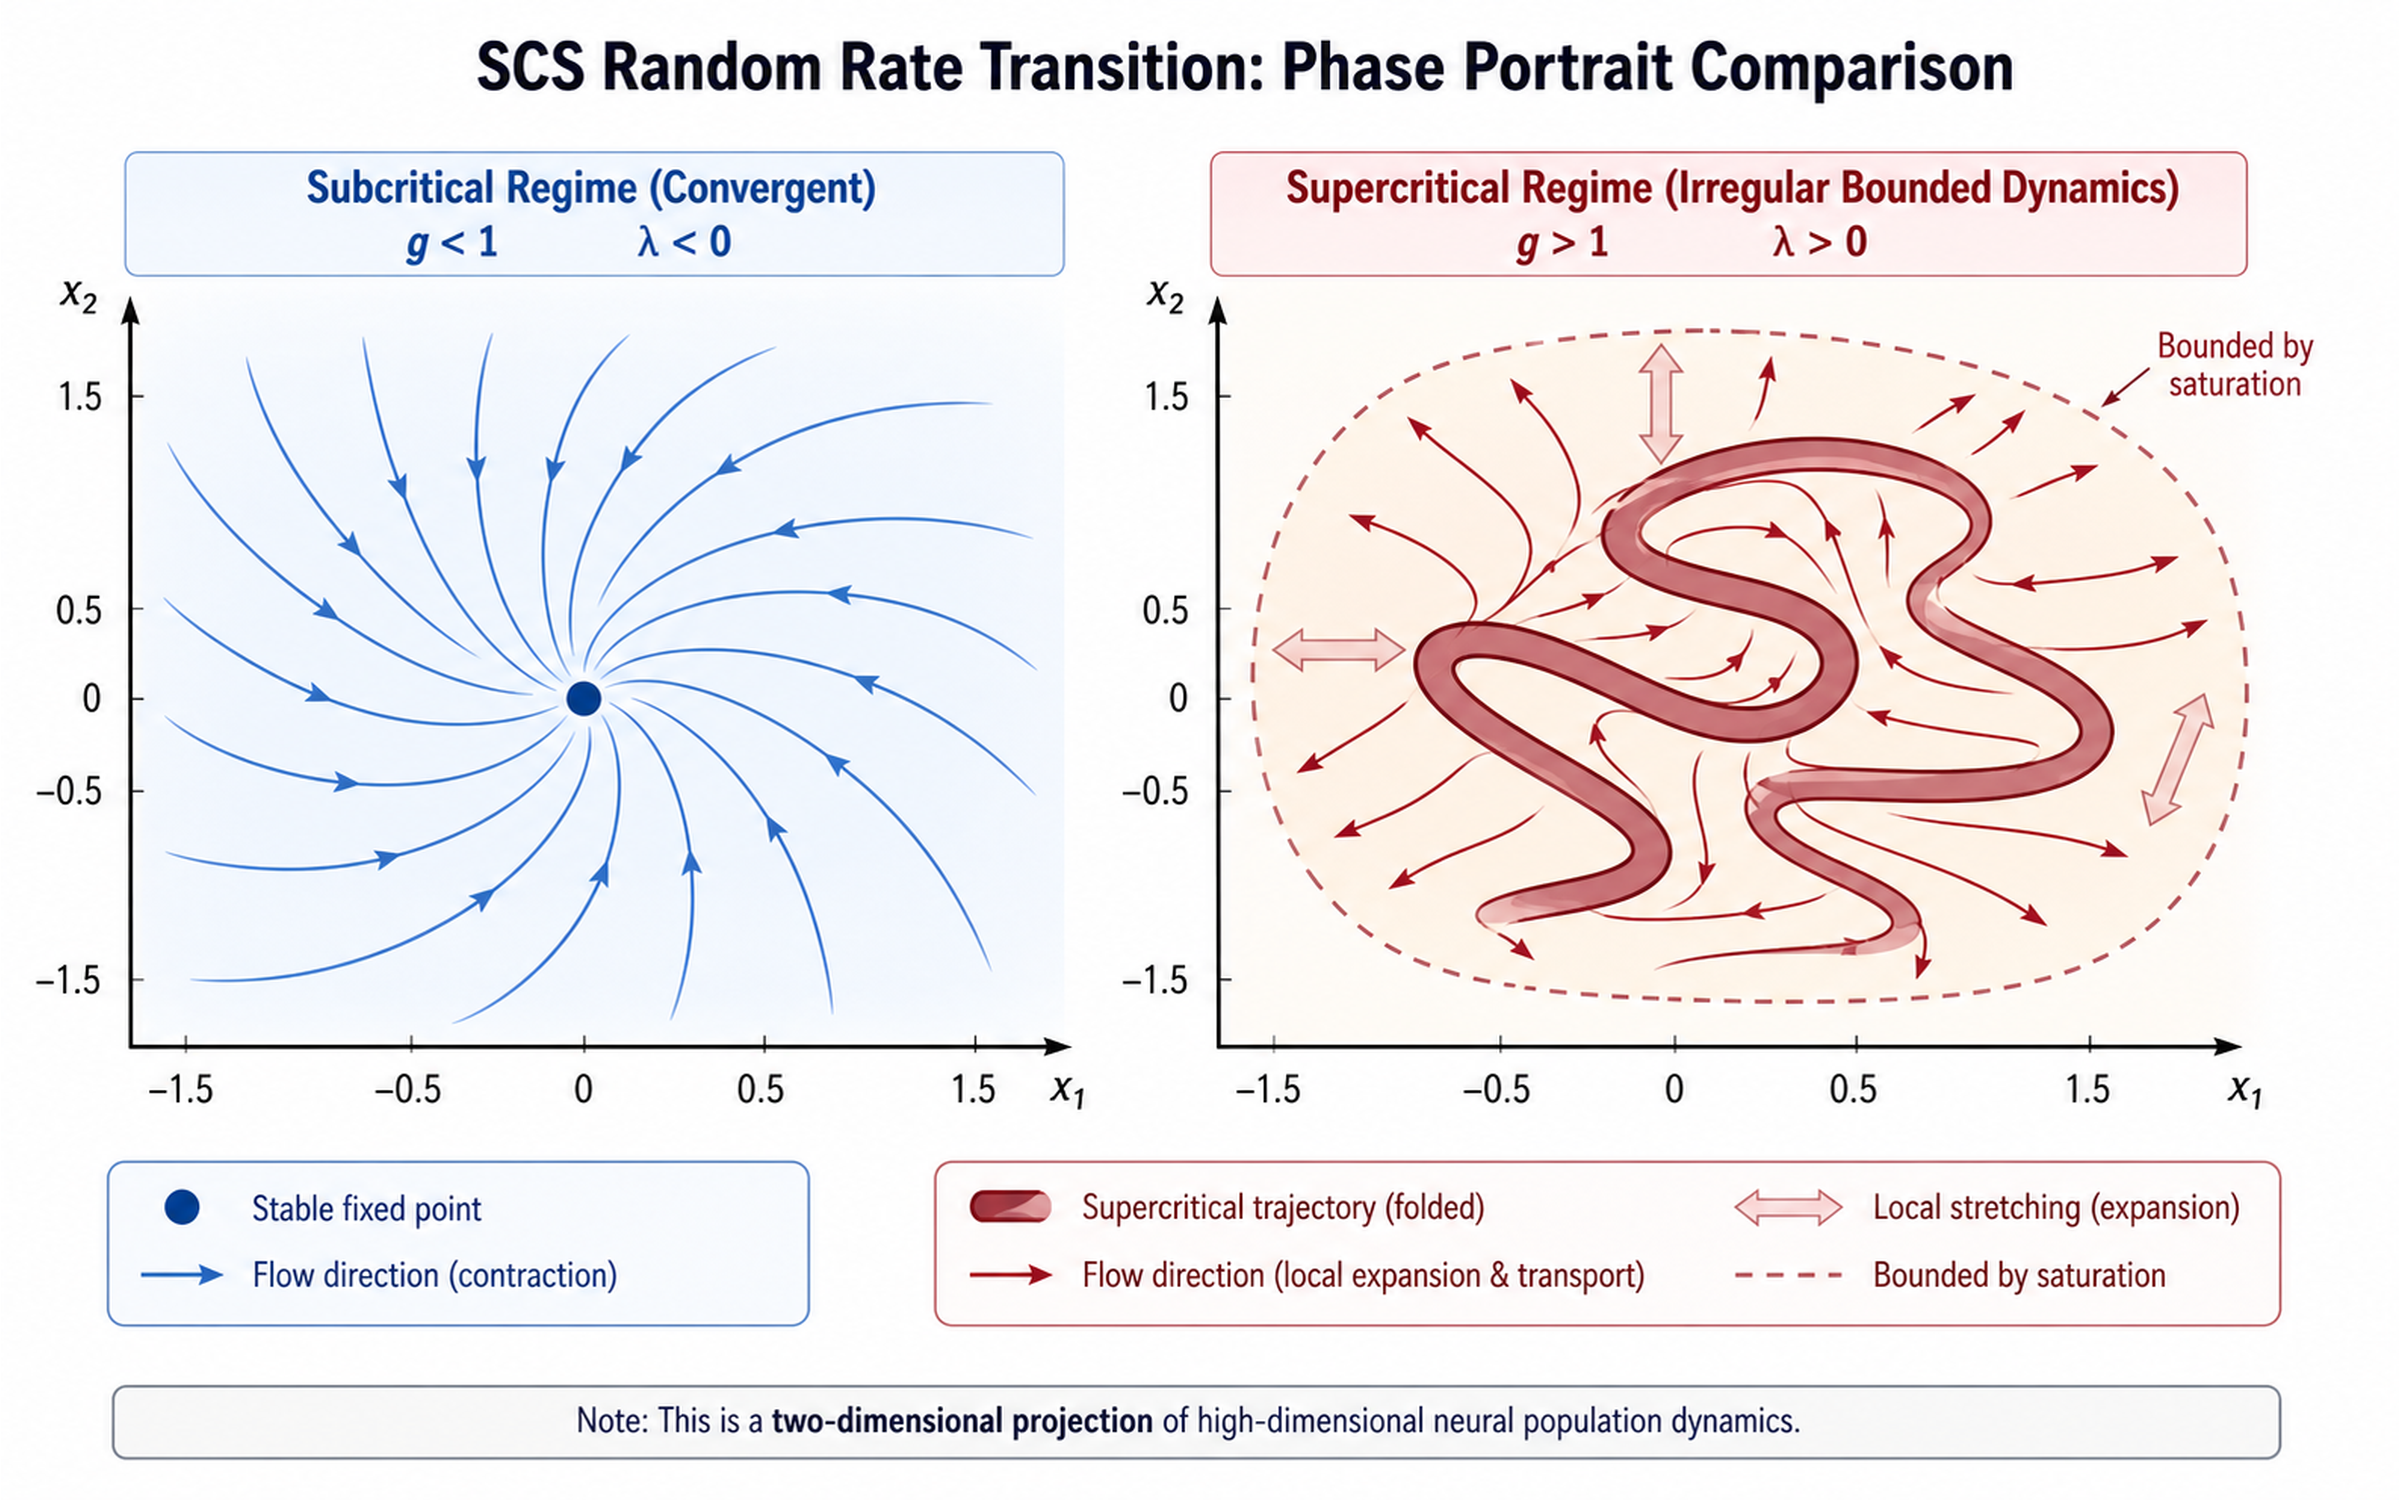
\includegraphics[width=0.88\textwidth]{figures/imagegen/ch06-random-rate-phase-portrait-img.png}
    \caption{Random rate dynamics before and after the SCS instability. The
    left panel represents contraction toward a stable fixed point when recurrent
    gain is below the leak. The right panel represents expansion, folding, and
    bounded irregular motion after the random gain crosses the critical value.
    The picture is schematic: the true SCS state space is high-dimensional, but
    the mathematical point is the competition between leak and random recurrent
    amplification.}
    \label{fig:ch06-random-rate-phase-portrait}
\end{figure}

\section{The SCS Transition as a Self-Consistency Problem}
\label{sec:ch06-scs-self-consistency}

The SCS transition is deeper than the linear instability calculation. In a large
random network, the recurrent input to a typical unit is a sum of many weak
random terms,
\[
        h_i(t) = \sum_{j=1}^{N} J_{ij}\,\phi(x_j(t)).
\]
For large \(N\), and under the standard weak-correlation assumptions of random
network mean-field theory, this input behaves like a Gaussian process by a
central-limit argument. The catch is that its covariance is generated by the
same network activity it drives. This is the self-consistency structure.

Define the rate autocovariance
\[
        C_r(\tau)
        =
        \left\langle \phi(x(t))\phi(x(t+\tau))\right\rangle
        -
        \left\langle \phi(x(t))\right\rangle^2 ,
        \label{eq:ch06-rate-autocovariance}
\]
where the brackets denote averaging over time, units, and disorder in the
stationary regime. In the zero-mean SCS model,
\[
        \left\langle h_i(t)h_i(t+\tau)\right\rangle
        =
        g^2 C_r(\tau).
        \label{eq:ch06-scs-input-covariance}
\]
The factor \(g^2\) comes from the variance of the couplings.
Equation~\eqref{eq:ch06-scs-input-covariance} says that the random network converts the
output autocorrelation into input autocorrelation.

A representative unit is therefore described by
\[
        \tau_r \frac{d x}{dt} = -x(t) + \eta(t),
        \label{eq:ch06-scs-effective-unit}
\]
where \(\eta(t)\) is a zero-mean Gaussian process whose covariance must satisfy
\[
        \left\langle \eta(t)\eta(t+\tau)\right\rangle = g^2 C_r(\tau).
        \label{eq:ch06-effective-noise-covariance}
\]
The effective unit is not driven by arbitrary external noise. It is driven by a
noise process whose statistics are generated by the network itself. The
self-consistency condition closes the loop:
\[
        C_r(\tau)
        =
        \left\langle \phi(x(t))\phi(x(t+\tau))\right\rangle
        -
        \left\langle \phi(x(t))\right\rangle^2,
        \quad
        x(t)\ \hbox{solves}\ \eqref{eq:ch06-scs-effective-unit}.
        \label{eq:ch06-scs-self-consistency}
\]

This is why the transition is not diagnosed only by watching a simulated trace.
One asks whether the self-consistency equations admit a nontrivial stationary
autocorrelation. Below threshold the only stable solution is the quiescent or
fixed-point solution. Above threshold there is a nonzero, time-dependent
autocorrelation corresponding to deterministic chaos.

\section{Autocorrelations Across the Transition}
\label{sec:ch06-autocorrelation-transition}

Autocorrelation is the key observable because it turns irregular time series
into a reproducible statistical object. For the effective linear
filter~\eqref{eq:ch06-scs-effective-unit}, the input covariance and the activation
covariance \(C_x(\tau)\) obey
\[
        \left(1-\tau_r^2\frac{d^2}{d\tau^2}\right)C_x(\tau)
        =
        g^2 C_r(\tau),
        \label{eq:ch06-autocorrelation-filter}
\]
with
\[
        C_r(\tau)
        =
        \left\langle \phi(x(t))\phi(x(t+\tau))\right\rangle
        -
        \left\langle \phi(x(t))\right\rangle^2 .
\]
The left side is the effect of leak: a white or fast input is smoothed by the
rate time constant. The right side is the recurrent source of fluctuations.

As \(g\) increases, three qualitative changes occur.

\begin{enumerate}
    \item For \(g<g_c\), perturbations decay and the autocorrelation of
    internally generated fluctuations is trivial in the deterministic infinite
    network.
    \item Near \(g_c\), the leading decay rate becomes small. Correlations
    broaden because the network almost balances leak in its most unstable
    directions.
    \item For \(g>g_c\), the chaotic state has a smooth autocorrelation whose
    width gives the characteristic timescale of the macroscopic irregular
    activity.
\end{enumerate}

The subcritical curve in Figure~\ref{fig:ch06-scs-autocorrelation-transition}
should therefore be read as a decay or response timescale, for example the
relaxation of a small perturbation or the autocorrelation produced when small
external or finite-size fluctuations are present. In the deterministic
infinite-size SCS model below threshold, there is no self-sustained chaotic
autocorrelation.

The smoothness at zero lag matters for the later distinction between chaos and
finite-size switching. A purely deterministic chaotic rate process has
\(C_r' (0)=0\) under the usual stationary smoothness assumptions. By contrast,
finite-size spike-count noise can contribute an Ornstein--Uhlenbeck-like term
proportional to \(e^{-|\tau|/\tau_\xi}\), which produces a kink at zero lag.
The zero-lag shape is therefore not just a plotting detail; it encodes the
source of variability.

\begin{figure}[htbp]
    \centering
    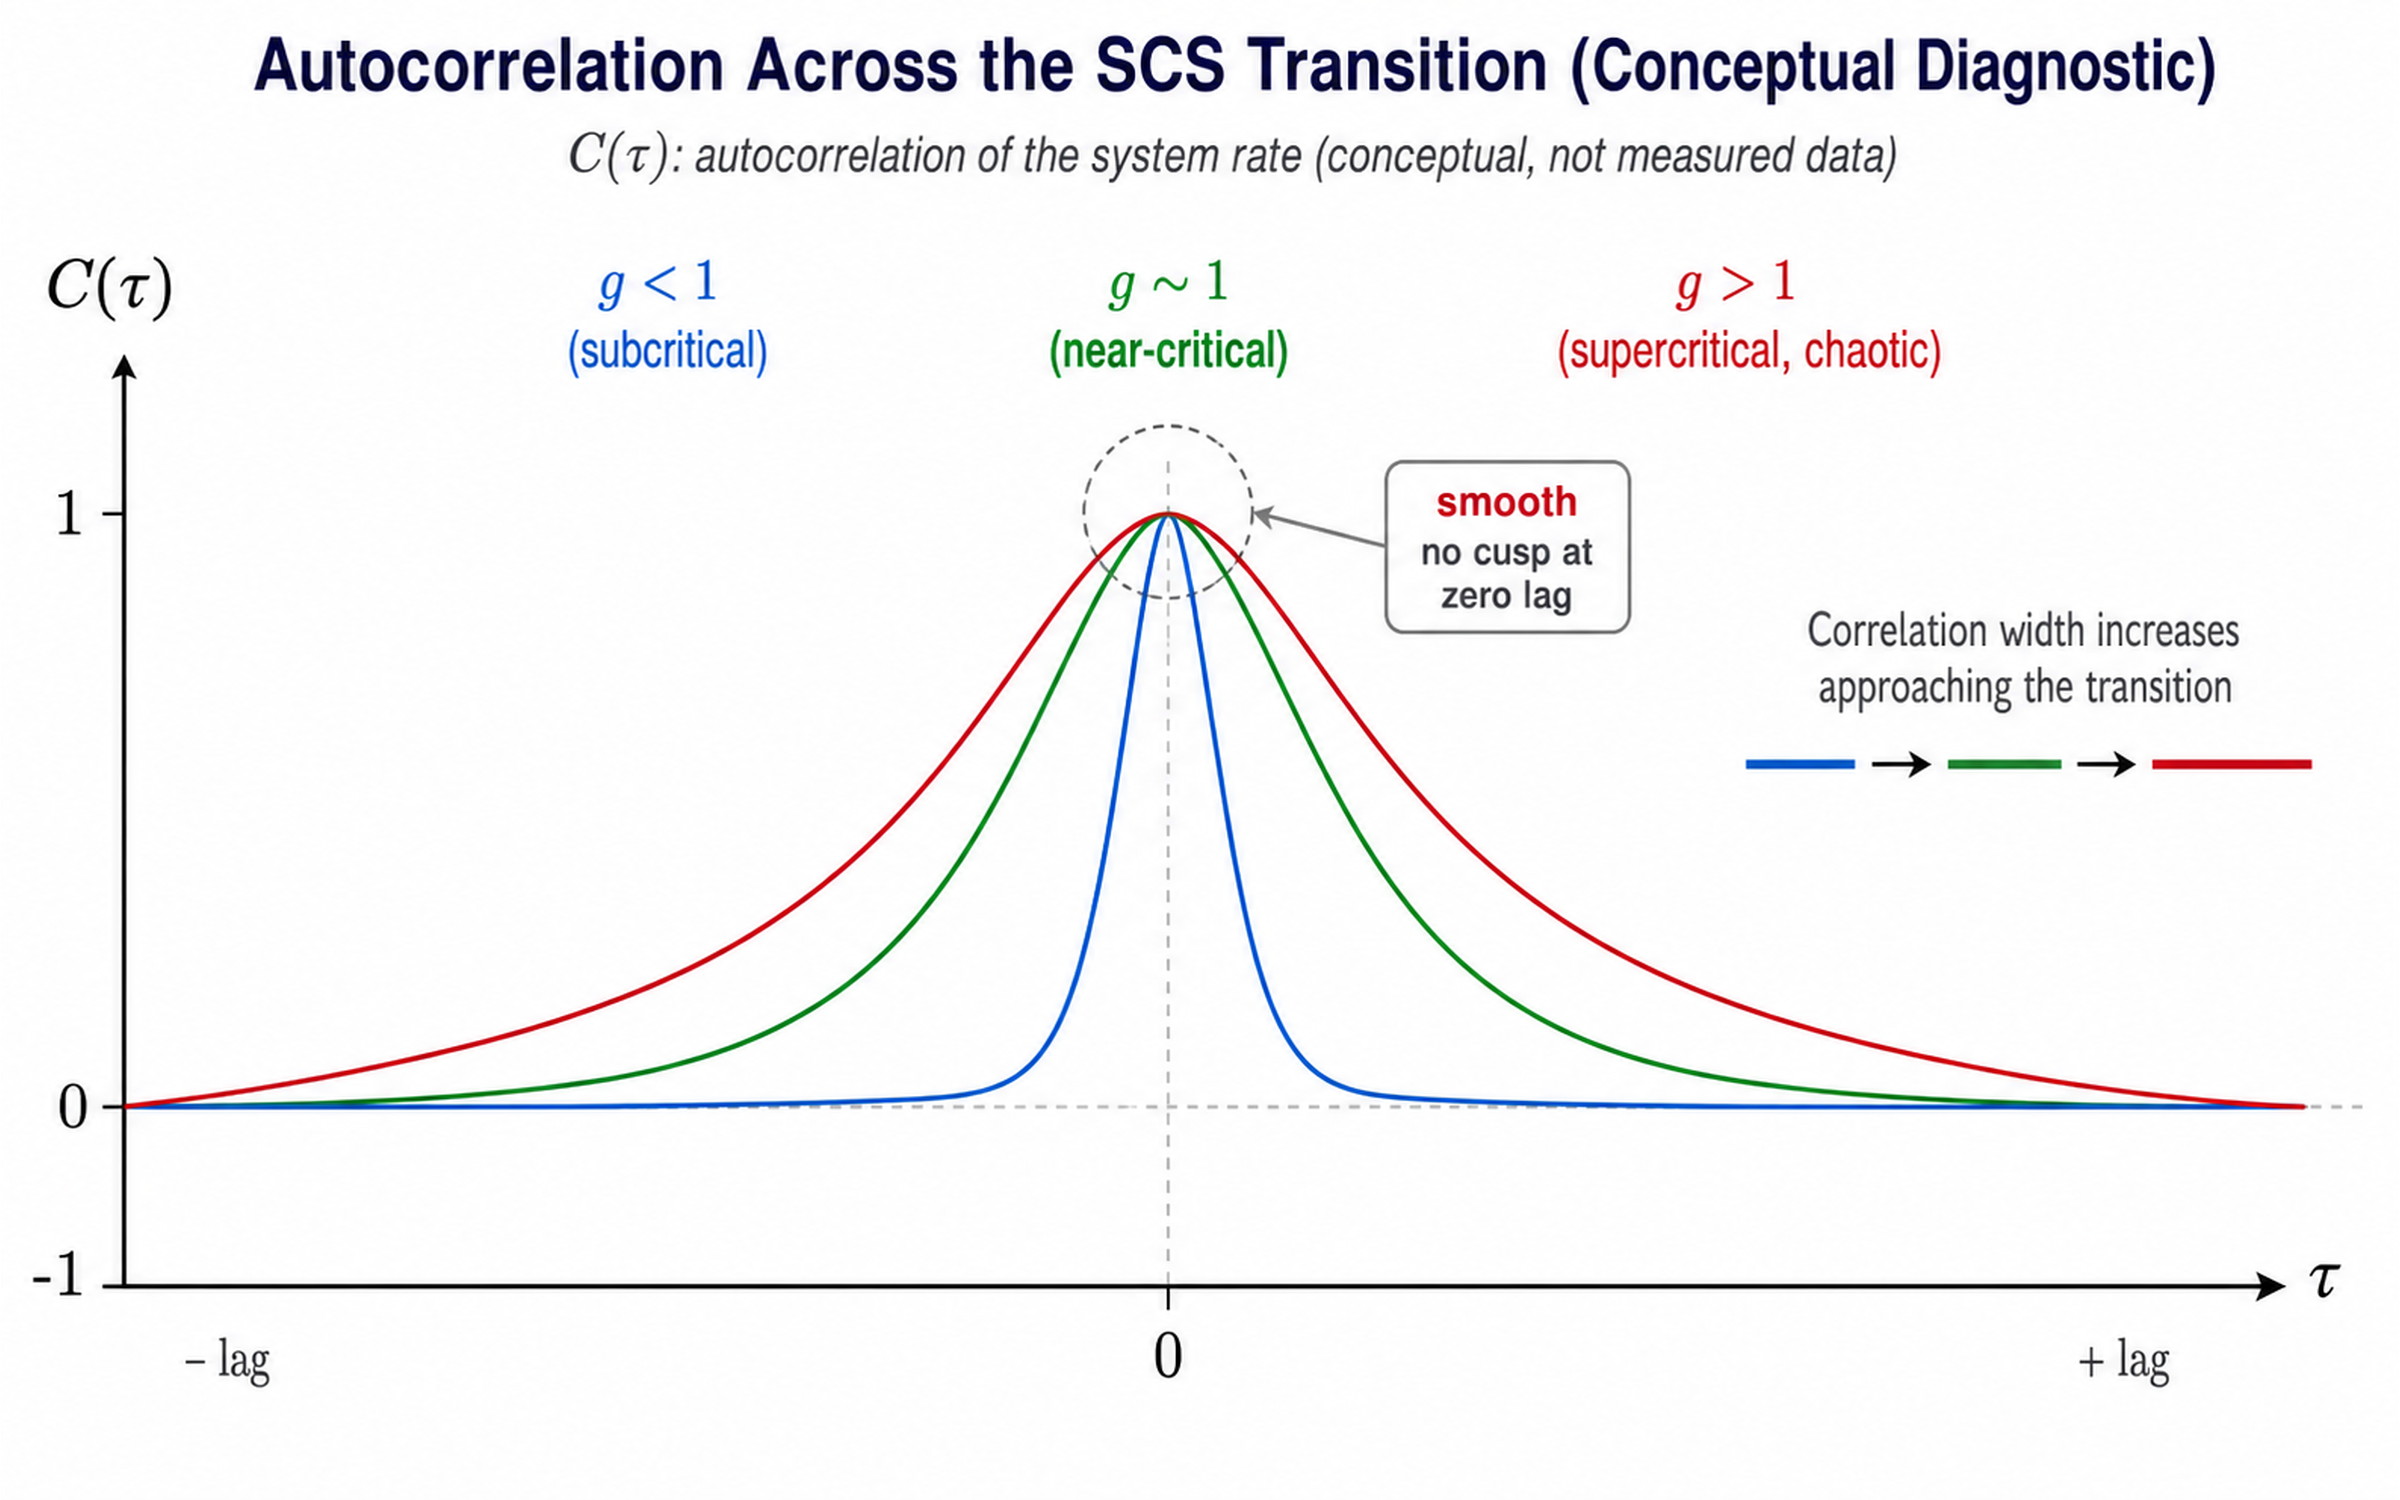
\includegraphics[width=0.88\textwidth]{figures/imagegen/ch06-scs-autocorrelation-transition-img.png}
    \caption{Autocorrelation as a diagnostic of the SCS transition. Below the
    transition, internally generated deterministic fluctuations contract. Near
    criticality, correlations broaden because recurrent gain nearly cancels
    leak. Above the transition, the chaotic autocorrelation is smooth at zero
    lag and its half-width measures the macroscopic timescale. A finite-size
    noise contribution would add a sharper zero-lag kink rather than the smooth
    chaotic shoulder shown here.}
    \label{fig:ch06-scs-autocorrelation-transition}
\end{figure}

\section{Lyapunov Diagnostics}
\label{sec:ch06-lyapunov}

The second diagnostic of chaos is sensitivity to initial conditions. Let
\(\delta x_i(t)\) be the difference between two nearby trajectories evolving in
the same frozen network. Linearizing along a trajectory gives
\[
        \tau_r \frac{d\,\delta x_i}{dt}
        =
        -\delta x_i(t)
        +
        \sum_{j=1}^{N}J_{ij}\,\phi'(x_j(t))\,\delta x_j(t).
        \label{eq:ch06-tangent-dynamics}
\]
The largest Lyapunov exponent is
\[
        \lambda_{\max}
        =
        \lim_{t\to\infty}
        \frac{1}{t}
        \log\frac{\|\delta x(t)\|}{\|\delta x(0)\|}.
        \label{eq:ch06-lyapunov}
\]
If \(\lambda_{\max}<0\), perturbations decay. If
\(\lambda_{\max}>0\), nearby trajectories separate exponentially until
nonlinearity folds them back into the bounded state space. This is why a
perturbation test can distinguish metastability from chaos. In a multistable
attractor landscape, a small perturbation inside a basin relaxes back to the
same attractor. In a chaotic rate state, an arbitrarily small perturbation along
an expanding direction changes the future trajectory, even though macroscopic
statistics such as \(C_r(\tau)\) remain stationary.

\begin{figure}[htbp]
    \centering
    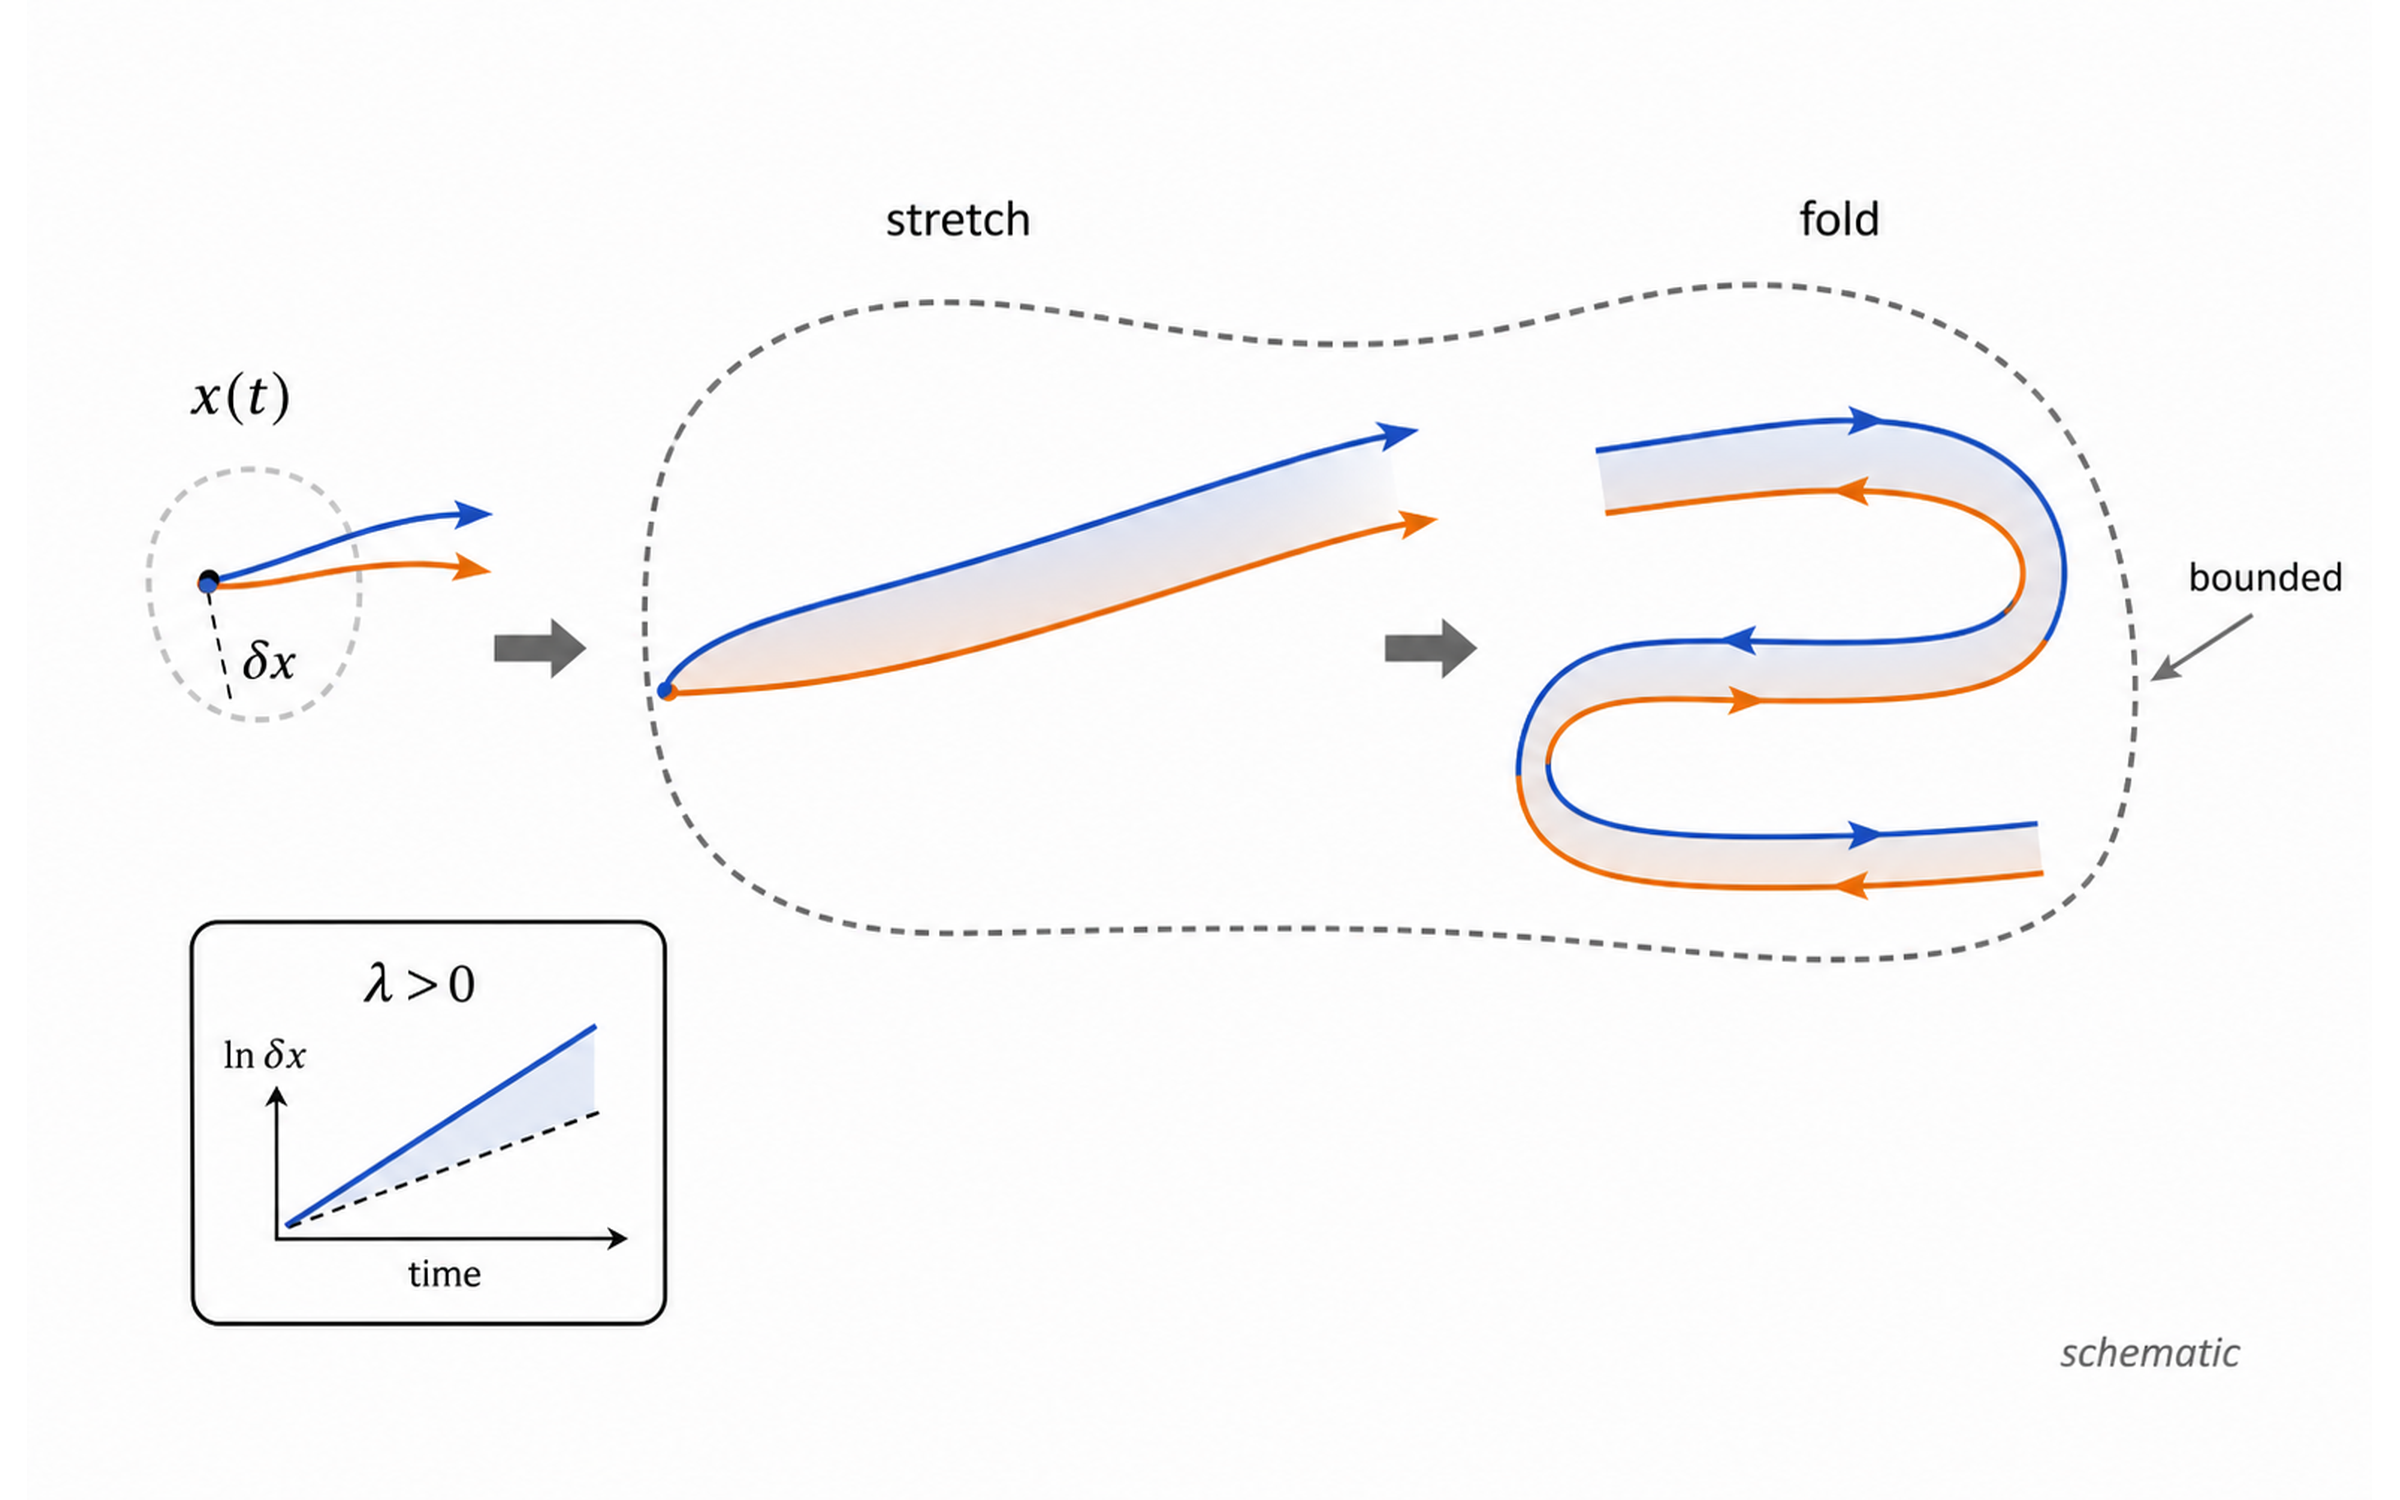
\includegraphics[width=0.88\textwidth]{figures/imagegen/ch06-chaotic-flow-folding-img.png}
    \caption{The geometric mechanism behind a positive Lyapunov exponent. Nearby states separate along locally expanding directions, while the nonlinear transfer function and leak keep the motion bounded by folding trajectories back into the accessible state space. Chaos is the coexistence of local divergence and global confinement, not unbounded rate growth.}
    \label{fig:ch06-chaotic-flow-folding}
\end{figure}

\section{Turning SCS into Diagnostics}
\label{sec:ch06-scs-diagnostics}

The SCS model is useful here because it gives a checklist for clustered
simulations, not because the spiking network literally has independent Gaussian
rate weights. The checklist is:

\begin{keyequation}[SCS Diagnostic Translation]
\begin{center}
\renewcommand{\arraystretch}{1.35}
\begin{tabularx}{\textwidth}{@{}l X X@{}}
  \toprule
  \textbf{SCS object} & \textbf{Clustered-network analogue} & \textbf{Diagnostic use} \\
  \midrule
  \(g\phi'(0)\) or spectral radius &
  Local tangent gain of the filtered cluster-rate equations &
  Locate candidate transition regions before expensive Lyapunov scans \\
  \(C_r(\tau)\) self-consistency &
  Cluster-rate autocovariance reproduced by effective input statistics &
  Test whether a reduced theory predicts the observed timescale \\
  Smooth \(C_r(\tau)\) at zero lag &
  Smooth shoulder in filtered cluster-rate autocorrelation &
  Separate deterministic rate variability from finite-size OU-like kinks \\
  Frozen random matrix \(J\) &
  Quenched inter-cluster weights, sparse adjacency, or heterogeneous depression &
  Keep the same realization in perturbation and scaling tests \\
  \(N\to\infty\) rate limit &
  Many large clusters with \(\xi\to0\) but nonzero aggregate \(\kappa\) &
  Ask whether switching survives without finite-size spike-count noise \\
  \bottomrule
\end{tabularx}
\end{center}
\end{keyequation}

The most common mistake is to replace this checklist by a visual comparison of
traces. Irregular switching can be produced by finite-size hopping among
attractors, by deterministic chaos, or by a mixture of both. SCS tells us which
statistics must be measured: tangent growth, autocorrelation width, zero-lag
shape, and scaling with the number of neurons per cluster.

\section{Self-Coupled and MAS-Type Rate Units}
\label{sec:ch06-mas-self-coupled}

The classical SCS unit has no explicit self-coupling other than the leak. A
clustered network suggests a slightly richer rate unit. A cluster can have strong
potentiated recurrent excitation and inhibition inside itself, so its effective
rate equation may contain a self-coupling term:
\[
        \tau_c \frac{d u_a}{dt}
        =
        -u_a(t)
        + w_{\mathrm{self}}\,\Phi(u_a(t))
        + \sum_{b\ne a} G_{ab}\,\Phi(u_b(t))
        + I_a .
        \label{eq:ch06-self-coupled-rate}
\]
Here \(a\) labels clusters, \(u_a\) is the effective drive of cluster \(a\),
\(\Phi\) is a cluster transfer function, \(w_{\mathrm{self}}\) summarizes
within-cluster potentiation, and \(G_{ab}\) summarizes inter-cluster coupling.
In the roadmap, ``MAS'' refers to the Merav Stern--Haim
Sompolinsky--L. F. Abbott style analogy: random networks of bistable or
self-coupled units whose collective dynamics can undergo a transition to chaos.
The analogy is useful because the cluster-level variable in
Equation~\eqref{eq:ch06-self-coupled-rate} can behave like a deterministic
rate unit with internal positive feedback.

The analogy should not be read as an identity of microscopic models. In the
clustered spiking model, the self-coupling is produced by potentiated
within-cluster E/I synapses, while the couplings between clusters have their
own depression, signs, sparsity, and quenched heterogeneity. Thus MAS-type
language names the self-coupled-unit intuition, not a claim that the clustered
spiking network has the same coupling matrix as the original self-coupled rate
model.

Self-coupling changes the local shape of the dynamics. With sufficiently strong
\(w_{\mathrm{self}}\), a single isolated unit may have a low-rate and a high-rate
state. Random inter-unit coupling then couples these local states into a
large recurrent system. Depending on parameters, the result can be stable
attractors, long transients, switching among quasi-stable configurations, or
chaos. This is the bridge from a pure SCS model to clustered spiking networks:
the cluster is not just a linear rate unit; it can have internal attractor-like
structure.

\section{Cluster Activities as Effective Rate Units}
\label{sec:ch06-cluster-rate-units}

For a clustered spiking network, the natural effective variable is the filtered
population activity of a cluster. If cluster \(a\) contains \(n_E\) excitatory
neurons in the local per-cluster sense, its excitatory activity can be written
schematically as
\[
        A_a^E(t)
        =
        \frac{1}{n_E}\sum_{j=1}^{n_E}s_{a,j}^E(t),
        \qquad
        r_a^E(t)
        =
        (\epsilon * A_a^E)(t),
        \label{eq:ch06-cluster-activity}
\]
where \(s_{a,j}^E(t)\) is the spike train of neuron \(j\) in cluster \(a\),
\(\epsilon\) is a synaptic or smoothing kernel, and \(*\) denotes convolution.
The variable \(r_a^E(t)\) is continuous enough to compare with a rate unit.

A minimal cluster-level rate reduction has the form
\[
        \tau_c \frac{d u_a}{dt}
        =
        -u_a
        +
        \widehat J\,\Phi(u_a)
        +
        \sum_{b\ne a}\check J_{ab}\,\Phi(u_b)
        +
        I
        +
        \xi\,\zeta_a(t).
        \label{eq:ch06-cluster-rate-reduction}
\]
The term \(\widehat J\) represents intra-cluster potentiation. The terms
\(\check J_{ab}\) represent inter-cluster weights. They can include both the
deterministic inter-cluster depression required to compensate for stronger
within-cluster coupling and a frozen heterogeneous part:
\[
        \check J_{ab}
        =
        \check J_{0}
        +
        \kappa\,\Delta_{ab},
        \qquad
        \left\langle \Delta_{ab}\right\rangle=0 .
        \label{eq:ch06-check-j-kappa}
\]
The coefficient \(\kappa\) is the quenched-disorder coordinate that will return
in Chapter~\ref{ch:mean-field-dynamic-mean-field-theory}. It is distinct from
the finite-size amplitude
\[
        \xi = \frac{1}{\sqrt{n_E}}
        \label{eq:ch06-xi-definition}
\]
which records the fact that a cluster rate is an average over finitely many spiking
neurons. The process \(\zeta_a(t)\) is not the SCS source of chaos; it is the
residual fluctuation from finite cluster size.

This equation should be read carefully. It does not say that spiking details
have disappeared. They have moved into \(\Phi\), \(\tau_c\), \(\xi\), the
autocorrelation of \(\zeta_a\), and the effective weights \(\widehat J\) and
\(\check J_{ab}\). The rate reduction is useful precisely because it lets us ask
which part of switching is due to finite-size fluctuations and which part is due
to deterministic, quenched-disorder-driven chaos.

\section{The SCS-to-Cluster Dictionary}
\label{sec:ch06-scs-cluster-dictionary}

The bridge to the paired E/I model is a controlled analogy. The dictionary is:
\[
\begin{array}{rcl}
  \hbox{SCS unit } i
  &\longleftrightarrow&
  \hbox{paired cluster } a,\\[2pt]
  x_i(t)
  &\longleftrightarrow&
  u_a(t)\hbox{ or }(r_a^E(t),r_a^I(t)),\\[2pt]
  J_{ij}
  &\longleftrightarrow&
  \check J_{ab}^{\alpha\beta}\hbox{ and its cluster-level reduction},\\[2pt]
  g^2
  &\longleftrightarrow&
  \hbox{aggregate variance of quenched inter-cluster input},\\[2pt]
  C_r(\tau)
  &\longleftrightarrow&
  C_{ab}^{\alpha\beta}(\tau)
  =
  \langle r_a^\alpha(t)r_b^\beta(t+\tau)\rangle
  -
  \langle r_a^\alpha\rangle\langle r_b^\beta\rangle .
\end{array}
\]
The dictionary has two limits. First, the cluster must be large enough that a
filtered population rate is a meaningful state variable; otherwise
\(\xi\)-driven spike-count noise dominates the measurement. Second, the number
of effective units must be large enough for a random-network mean-field picture
to be sensible; a handful of clusters can have sample-specific dynamics but not
a clean SCS thermodynamic limit.

In the many-large-cluster regime, the deterministic part of a cluster-rate
model can inherit SCS-like behavior. In a fixed-cluster-size regime, the same
autocorrelation width may instead come from finite-size hopping. The practical
task is therefore comparative: hold the quenched inter-cluster realization
fixed, increase \(n_E\) and \(n_I\) inside each cluster, and ask which
statistics persist as \(\xi\) decreases.

\section{What Carries Forward}
\label{sec:ch06-carries-forward}

Chapter~\ref{ch:mean-field-dynamic-mean-field-theory} generalizes the
self-consistency logic from the SCS rate network to clustered spiking and
cluster-level reductions. The essential ideas to carry forward are these:

\begin{enumerate}
    \item A high-dimensional random recurrent sum can become an effective
    Gaussian process for a representative unit.
    \item The covariance of that process is not externally chosen; it must match
    the autocorrelation generated by the representative unit.
    \item The SCS transition is controlled by recurrent gain, diagnosed by
    autocorrelation shape and by the largest Lyapunov exponent.
    \item Cluster activities can play the role of rate units, but finite-size
    noise \(\xi\) and quenched inter-cluster variability \(\kappa\) must remain
    separate in the theory.
\end{enumerate}

\begin{chaptersummary}
\begin{center}
\renewcommand{\arraystretch}{1.35}
\begin{tabularx}{\textwidth}{@{}l X X@{}}
  \toprule
  \textbf{Object} & \textbf{Formula} & \textbf{Research use} \\
  \midrule
  Random scaling &
  \(J_{ij}=g\chi_{ij}/\sqrt{N}\) &
  Keeps recurrent random input order one in the many-unit limit \\
  Linear threshold &
  \(g\phi'(0)=1\) &
  First estimate of the rate-chaos transition \\
  Effective covariance &
  \(\langle \eta(t)\eta(t+\tau)\rangle=g^2C_r(\tau)\) &
  Turns an irregular trace into a self-consistency problem \\
  Tangent dynamics &
  \(\tau_r\dot{\delta x}_i=-\delta x_i+\sum_j J_{ij}\phi^{\prime}(x_j)\delta x_j\) &
  Defines the Lyapunov test for deterministic sensitivity \\
  Cluster reduction &
  \(\tau_c\dot u_a=-u_a+\widehat J\Phi(u_a)+\sum_{b\ne a}\check J_{ab}\Phi(u_b)+I+\xi\zeta_a\) &
  Separates self-coupling, quenched inter-cluster structure, and finite-size noise \\
  \bottomrule
\end{tabularx}
\end{center}
\end{chaptersummary}

\section{Contribution-Level Checkpoints}
\label{sec:ch06-contribution-checkpoints}

\begin{enumerate}
    \item Derive \cref{eq:ch06-linearized-rate} and
    \cref{eq:ch06-local-gain-cluster} from the nonlinear rate equations. Then
    compute the empirical spectral radius of the random block in a simulated
    cluster-level connectivity matrix and compare it with the observed onset of
    broad cluster-rate autocorrelations.

    \item Simulate the SCS rate network for several values of \(g\). For each
    value, estimate \(C_r(\tau)\), its half-width at half-maximum, and the
    largest Lyapunov exponent using the tangent equation. Record which
    diagnostic changes first near \(g_c\).

    \item Take a filtered cluster-rate trace from a spiking simulation and fit
    two short-lag models: a smooth even function and a smooth function plus
    \(A_\xi e^{-|\tau|/\tau_\xi}\). Use the fitted \(A_\xi\) across cluster
    sizes to test whether the zero-lag kink scales like finite-size noise.

    \item Build the SCS-to-cluster dictionary for one concrete E/I model:
    identify the effective unit, the self-coupling, the quenched random block,
    the finite-size noise source, and the observable that plays the role of
    \(C_r(\tau)\).
\end{enumerate}
